% Drawing 137/02-1 -- folder 137, batch 02, archive page 22 (PDF page 23).
% Transcription: sous cette suite, un croquis : $\Phi^{i-1} \xrightarrow{u} \Psi^{i-1}$ (flèche montante), des obliques $\partial_{i-1}$ vers $\Phi^{i}$ et $\partial_i$ de $\Phi^{i}$ vers $\Phi^{i+1}$, et une flèche descendante $\Psi^{i} \hookrightarrow \Phi^{i+1}$
% Kind: sketch around the exact sequence (*): u, d_{i-1}, d_i. Method 2 (schematic redraw from the facsimile). Status: ok.
% Notes: Under the sequence (*) (redrawn with it for position: 0 - Psi^{i-1} => Phi^i -> Psi^i -> 0), the sketch: Phi^{i-1} -u-> Psi^{i-1} (upward arrow, double head), the oblique d_{i-1} from Phi^{i-1} towards Phi^i, the oblique d_i from Phi^i down to the right, and a downward arrow from Psi^i to Phi^{i+1}.
% Coordinates: 1 unit = 1 mm = 1/100 of the crop width (bbox in page fractions: [0.18, 0.32, 0.42, 0.4]).
% Redrawn by Claude (claude-opus-5-5), issue #73, 2026-11-07; not checked by a human; not compiled (no TeX in the session).
% Rights: reproduces part of the work -- behind RENDER_TRANSCRIPTS, never published by itself.
\documentclass[tikz,border=3pt]{standalone}
\usepackage{amsmath,amssymb}
\usetikzlibrary{patterns,arrows.meta}
\tikzset{pencil/.style={black!45}, struck/.style={black!35}, mark/.style={circle,draw,inner sep=1.3pt}, pt/.style={circle,fill,inner sep=0.9pt}, opt/.style={circle,draw,fill=white,inner sep=1.1pt}}
\begin{document}
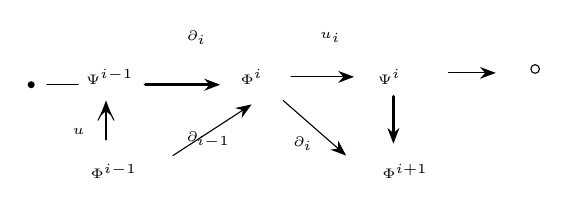
\begin{tikzpicture}[x=1mm,y=1mm,line cap=round,line join=round,font=\scriptsize]
\node[pt] at (14,-14) {};
\draw (16,-14) -- (20,-14);
\node[inner sep=1pt] at (24,-13) {\tiny $\Psi^{i-1}$};
\draw[-{Stealth[length=2mm]},very thick] (28.5,-14) -- (38,-14);
\node[inner sep=1pt] at (35,-8) {\tiny $\partial_i$};
\node[inner sep=1pt] at (42,-13) {\tiny $\Phi^{i}$};
\draw[-{Stealth[length=2mm]}] (47,-13) -- (55,-13);
\node[inner sep=1pt] at (52,-8) {\tiny $u_i$};
\node[inner sep=1pt] at (59.5,-13) {\tiny $\Psi^{i}$};
\draw[-{Stealth[length=2mm]}] (67,-12.5) -- (73,-12.5);
\node[opt] at (78,-12) {};
\node[inner sep=1pt] at (24.5,-25) {\tiny $\Phi^{i-1}$};
\draw[-{Stealth[length=2mm]}] (23.5,-21) -- (23.5,-16);
\draw (22.5,-18.5) -- (23.5,-16.5) -- (24.5,-18.5);
\node[inner sep=1pt] at (20,-20) {\tiny $u$};
\draw[-{Stealth[length=2mm]}] (32,-23) -- (42,-16.5);
\node[inner sep=1pt] at (36.5,-21) {\tiny $\partial_{i-1}$};
\draw[-{Stealth[length=2mm]}] (46,-16) -- (54,-23);
\node[inner sep=1pt] at (48.5,-21.5) {\tiny $\partial_i$};
\draw[-{Stealth[length=2mm]},very thick] (60,-15.5) -- (60,-21.5);
\node[inner sep=1pt] at (61.5,-25) {\tiny $\Phi^{i+1}$};
\end{tikzpicture}
\end{document}
